\documentclass[tikz,border=4pt]{standalone}
\usetikzlibrary{positioning, fit, backgrounds, shapes.geometric, arrows.meta}

\tikzset{
  task/.style       = {draw, thick, rounded corners=2pt, fill=white,
                       minimum width=26mm, minimum height=9mm, align=center},
  choice/.style     = {draw, thick, diamond, aspect=2, inner sep=1pt,
                       fill=white, align=center},
  lane/.style       = {draw=gray!60, fill=gray!8, rounded corners=2pt, inner sep=3mm},
  lane title/.style = {font=\bfseries\small},
  >={Stealth[length=2.5mm]},
}

\begin{document}
% An expense claim in three lanes, one per role. Each lane fits its own
% steps and the two shared coordinates, so all three are as tall.
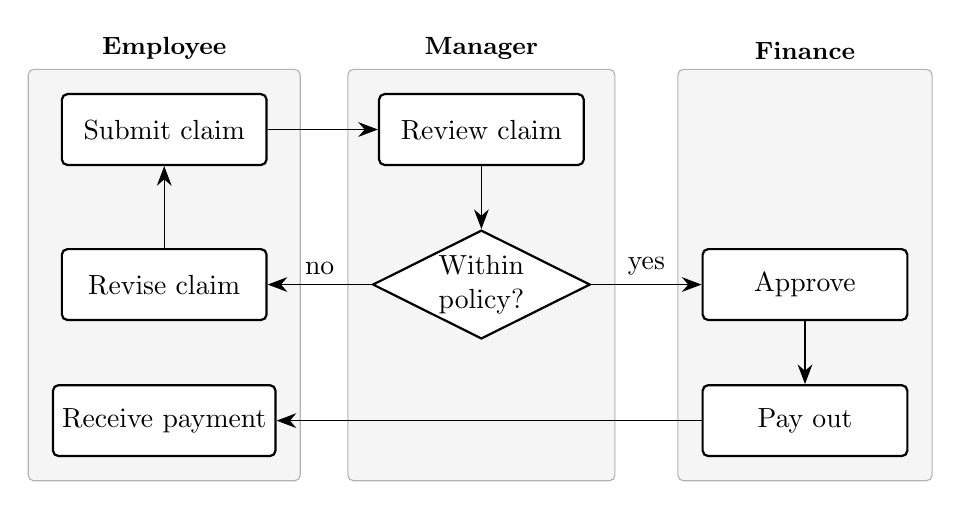
\begin{tikzpicture}[node distance=8mm and 14mm]
  \node[task]                      (submit)  {Submit claim};
  \node[task, right=of submit]     (review)  {Review claim};
  \node[choice, below=of review]   (policy)  {Within\\ policy?};
  \node[task] (revise) at (submit |- policy) {Revise claim};
  \node[task, right=of policy]     (approve) {Approve};
  \node[task, below=of approve]    (pay)     {Pay out};
  \node[task] (paid) at (submit |- pay)      {Receive payment};

  \draw[->] (submit)  -- (review);
  \draw[->] (review)  -- (policy);
  \draw[->] (policy)  -- node[above] {yes} (approve);
  \draw[->] (policy)  -- node[above] {no}  (revise);
  \draw[->] (revise)  -- (submit);
  \draw[->] (approve) -- (pay);
  \draw[->] (pay)     -- (paid);

  \begin{scope}[on background layer]
    \coordinate (lanes top) at (submit.north);
    \coordinate (lanes bottom) at (paid.south);
    \node[lane, fit=(submit) (revise) (paid) (submit |- lanes top) (submit |- lanes bottom),
          label={[lane title]north:Employee}] (employee) {};
    \node[lane, fit=(review) (policy) (review |- lanes top) (review |- lanes bottom),
          label={[lane title]north:Manager}] (manager) {};
    \node[lane, fit=(approve) (pay) (approve |- lanes top) (approve |- lanes bottom),
          label={[lane title]north:Finance}] (finance) {};
  \end{scope}
\end{tikzpicture}
\end{document}
